%\input{tcilatex}
%\input{tcilatex}


\documentclass[a4paper,10pt]{article}
%%%%%%%%%%%%%%%%%%%%%%%%%%%%%%%%%%%%%%%%%%%%%%%%%%%%%%%%%%%%%%%%%%%%%%%%%%%%%%%%%%%%%%%%%%%%%%%%%%%%%%%%%%%%%%%%%%%%%%%%%%%%%%%%%%%%%%%%%%%%%%%%%%%%%%%%%%%%%%%%%%%%%%%%%%%%%%%%%%%%%%%%%%%%%%%%%%%%%%%%%%%%%%%%%%%%%%%%%%%%%%%%%%%%%%%%%%%%%%%%%%%%%%%%%%%%
\usepackage{amsfonts}
\usepackage[utf8]{inputenc}
\usepackage{indentfirst}
\usepackage{times}
\usepackage[T1]{fontenc}
\usepackage[affil-it]{authblk}
\usepackage{authblk}
\usepackage{amssymb,amsmath,amsthm,ragged2e}
\usepackage{setspace,lipsum}
\usepackage[pdftex]{color,graphicx}
\usepackage{adjustbox}
\usepackage{lmodern,caption}
\usepackage{booktabs,array}
\usepackage{epstopdf}
\usepackage{array,longtable}
\usepackage[top=3cm, bottom=2cm, left=3cm, right=2cm]{geometry}
\usepackage{latexsym,hhline}
\usepackage[round]{natbib}
\usepackage[colorlinks=true,allcolors=blue]{hyperref}
\usepackage{setspace}
\usepackage{tikz,color,listings,float,booktabs,enumerate,multirow,multicol,subcaption}
\usepackage{parskip}
\usepackage{bigstrut,hyperref,tabularx,ctable,array,longtable,tikz}
\usepackage{rotating}
\usepackage[listings]{tcolorbox}
\usepackage{fancyheadings,xspace,amsmath,tikz-qtree}
\usepackage[labelfont=bf]{caption}
\usepackage{threeparttable}
\usepackage{standalone}
\usepackage[pdftex]{color,graphicx}

\setcounter{MaxMatrixCols}{10}
%TCIDATA{OutputFilter=LATEX.DLL}
%TCIDATA{Version=5.50.0.2953}
%TCIDATA{<META NAME="SaveForMode" CONTENT="1">}
%TCIDATA{BibliographyScheme=BibTeX}
%TCIDATA{LastRevised=Saturday, March 18, 2017 04:40:50}
%TCIDATA{<META NAME="GraphicsSave" CONTENT="32">}

\DeclareGraphicsRule{.tif}{png}{.png}{`convert #1 `dirname #1`/`basename #1 .tif`.png}
\newcommand{\otoprule}{\midrule[\heavyrulewidth]}
\newcolumntype{Z}{>{\centering\arraybackslash}X}
\onehalfspacing
\DeclareMathOperator{\diag}{diag}
\DeclareMathOperator{\Ima}{Im}
\DeclareCaptionLabelSeparator{horse}{:\quad}
\captionsetup{
labelsep = horse,
figureposition = bottom }
\setlength{\parindent}{15pt}
\hypersetup{
pdftitle={TITLE},
pdfauthor={AUTHOR},
pdfsubject={SUBJECT},
pdfkeywords={KEYWORD} {KEYWORD} {KEYWORD},
colorlinks=true,
linkcolor=blue,
citecolor=blue,
filecolor=magenta,
urlcolor=blue
}
%\newtheorem{theorem}{Theorem}
%\newtheorem{proposition}{Proposition}
%\newtheorem{lemma}{Lemma}
%\newtheorem{definition}{Definition}
\newtheorem{mydef}{Definition}
\newtheorem{mytheo}{Theorem}
\newtheorem{mycoro}{Corollary}
\newtheorem{mypro}{Proposition}
\newcommand{\R}{\mathbb R}
\newcommand{\Nat}{\mathbb N}
\newcommand{\C}{\mathbb C}
\newcommand{\Pstar}{\mathbb{P}^{\ast}}
\newcommand{\E}{\mathbb{E}}
\newcommand{\Var}{\mathrm{Var}}
\newcommand{\Cov}{\mathrm{Cov}}
\newcommand{\Expect}{{\rm I\kern-.3em E}}
\tcbuselibrary{listings,theorems}
\usetikzlibrary{matrix}
%\input{tcilatex}

\begin{document}

\title{Robust Portfolio Optimization with Multivariate Copulas: a Worst-Case CVaR approach}
\author[]{ Fernando A. B. Sabino da Silva\thanks{\texttt{Department of Statistics, Federal University of Rio Grande do Sul, Porto Alegre, RS 91509-900, Brazil, e-mail: dasilvafbs@gmail.com}; Corresponding author.}}
\author[]{Flavio A. Ziegelmann\thanks{\texttt{Department of Statistics, Federal University of Rio Grande do Sul, Porto Alegre, RS 91509-900, Brazil and CNPq, e-mail: flavioz@ufrgs.br}}}
\author[]{Cristina Tessari \thanks{\texttt{Finance Division, Columbia Business School, Columbia University, New York, NY 10027, USA,
			e-mail: ct2759@columbia.edu}}}
\affil[]{}
%\affil[2]{}
\date{}
\maketitle

\begin{abstract}
Using data from the S\&P 500 stocks from 1990 to 2015, we measure the downside market risk by Conditional Value-at-Risk (CVaR) subject to return constraints through the use of multidimensional mixed Archimedean copulas. We implement a dynamic investing viable strategy where the portfolios are optimized using three different length of rolling calibration windows. The out-of-sample performance is evaluated and compared against two benchmarks: a multidimensional Gaussian copula model and a constant mix portfolio. Our empirical analysis shows that the Mixed Copula-CVaR approach generates portfolios with better downside risk statistics for any rebalancing period and it is more profitable than the Gaussian Copula-CVaR and the $1/N$ portfolios for daily and weekly rebalancing. To cope with the dimensionality problem we select a set of assets that are the most diversified, in some sense, to the S\&P 500 index in the constituent set. The accuracy of the VaR forecasts is determined by how well they minimize a capital requirement loss function. In order to mitigate data-snooping problems, we apply a test for superior predictive ability to determine which model significantly minimizes this expected loss function. We find that the minimum average loss of the mixed Copula-CVaR approach is smaller than the average performance of the Gaussian Copula-CVaR.


\smallskip

\smallskip

 \textbf{Keywords:} Asset Allocation; Finance; Gaussian Copula; Linear Programming; Mixed Copula; Risk Management; S\&P 500; Scenarios; WCCVaR.

 \textbf{JEL Codes:} G11; G12; G17.
\end{abstract}

\makeatletter

\makeatother

\affil[1]{PPGE-UFRGS} \affil[2]{PPGE-UFRGS, PPGA-UFRGS}

%\date{July 25, 2016}

\section{Introduction}
 The seminal article ``Portfolio Selection'' published by  \citet*{markowitz1952} introduces the foundation for Modern Portfolio Theory (MPT) or mean-variance analysis. \citet*{markowitz1952} considered the problem of an agent who wishes to find the maximum (expected) return for a given level of risk or minimize the risk for a given level of return. He identified that, by diversifying a portfolio among investments that have different return patterns, investors can build such an efficient portfolio.

Quantile functions are commonly used for measuring the market risk of models with parameter uncertainty and variability. Portfolio optimization involving a mean-value-at-risk (mean-VaR) portfolio and the CVaR have been analyzed by \citet*{alexander2002} and \citet*{rockafellar2000}, respectively. Akin to the classical Markowitz portfolio, in these approaches we want to determine the weights that maximize the portfolio return for a specified VaR or CVaR at a given confidence level, or minimize these quantiles for a given confidence level subject to a fixed portfolio return.

On the other hand, \citet{artzner1999}, \citet*{szego2005} and \citet*{zhu2009worst} show that VaR has undesirable properties such as lack of sub-additivity and thus it is not a coherent measure. Furthermore, \citet*{uryasev2001} show that VaR may be a non-convex function with respect to portfolio weights, which can lead to multiple portfolio local solutions, but CVaR is coherent both for continuous and discrete distributions and it is also a convex function. In addition, they show that an outright optimization with respect to CVaR is numerically difficult due to the dependence of the CVaR on VaR. However, \citet*{rockafellar2000} report that VaR and CVaR can be computed simultaneously, introducing auxiliary risk measures. It can be used then in conjunction with scenario based optimization algorithms, reducing the problem to a linear programming problem, which allows us to optimize a portfolio with very large dimensions and stable numerical implementations. 

A well-known problem of the Markowitz model is its sensitivity to the input parameters. In practice, the implementation of strategies based on the risk-return trade-off remains a fundamental challenge in many areas of financial management, since estimation errors in the expected returns of the assets and the covariance matrix of these returns can significantly affect the asset allocations weights, no longer leading to an efficient portfolio. This issue can be overcome by employing robust optimization and worst case techniques \citep{benati2003,zhu2009worst,polak2010,fertis2012,kakouris14,polak2017} in which assumptions about the distribution of the random variable are relaxed, and thus, we obtain the optimal portfolio solution by optimizing over a prescribed feasible set and possible densities (a comprehensive survey can be found in \citealp{gabrel2014}). Finally, \citet*{kakouris14} show how copula-based models can be introduced in the Worst Case CVaR (WCVaR) framework. This approach is motivated by an investor's desire to be protected against the worst possible scenario.

In this paper, we employ the Worst-Case Copula-CVaR framework to compute optimal portfolios using linear programming. By following the procedure introduced by \citet*{kakouris14}, we investigate the use and usefulness of high-dimensional copulas without pair-copula constructions in financial risk management. We evaluate the out-of-sample performance of the Worst Case Copula-CVaR and compare the relative performance of this strategy to the Gaussian Copula-CVaR, to the naive $1/N$ (equally-weighted) portfolio, and to the S\&P 500 index in the long term in terms of wealth accumulation and downside risk.

The novel contribution of this paper is to select a diversified set of assets that can be useful during crises and tranquil periods, i.e., a portfolio that somehow involves hedging of decisions to protect the investors against any market conditions and evaluate the approaches using a high-dimensional Archimedean and Gaussian copula models without constructing hierarchical copulas. 

Our data set consists of daily data of adjusted closing prices of all shares that belong to S\&P 500 market index from July 2nd, 1990 to December 31st, 2015. We obtain the adjusted closing prices from Bloomberg. The data set sample encompasses 6,426 days and includes a total of 1,100 stocks over the whole period. We consider only stocks that are listed throughout a 48 plus 6-month period in the analysis, i.e., close to 500 stocks in each trading period. Moreover, we consider alternative portfolio rebalancing frequencies and return constraints. Returns are calculated in excess of a risk-free return.

To be effective in dealing with uncertainty, we select, among all listed assets in each formation period, a subset of fifty stocks based on the ranked sum of absolute deviations (the twenty-five largest and smallest) between the normalized daily closing prices deviations of the S\&P 500 index and all shares, adjusting them by dividends, stock splits and other corporate actions. By selecting a diversified cluster of assets that can be useful during crises and tranquil periods we address the issue of asset allocation considering the purpose of risk diversification. Indeed, this methodology can be adopted by different types of investors, from very defensive to very aggressive profiles. These stocks are then evaluated over the next six months. Our backtest results indicate that the Worst Case Copula-CVaR approach outperforms consistently the benchmark strategies in the long term in terms of downside risk measured by VaR, CVaR, and capital requirement loss. 

The remainder of the paper is structured as follows. In Section 2 we present a general review, notations and definitions of the CVaR and mean-variance optimization methodologies and extend them to our Worst Case framework through the use of appropriate allowable and uncertainty sets. The data we use is briefly discussed in Section 3. Section 4 summarizes the empirical results of the analysis, while Section 5 concludes and provides further ideas for research.

\section{Specifications of the Models under Analysis}

\subsection{Conditional Value-at-Risk}

 Let $Y$ be a stochastic vector standing for market uncertainties and $F_{Y}$ be its distribution function, i.e., $F_{Y}\left( u\right) =P\left( Y\leq u\right) $. Let also $F_{Y}^{-1}\left( v\right) =\inf \left\{ u:F_{Y}\left(u\right) \geq v\right\} $ be its right continuous inverse and assume that it has a probability density function represented by $p(y)$\footnote{This assumption can be relaxed \citep{uryasev2013}.}. Define the $VaR_{\beta }$\thinspace\ as the $\beta $-quantile by 
\begin{eqnarray}
VaR_{\beta }\left( Y\right) &=& \arg \min \left\{ \alpha \in\mathbb{R}:P\left( Y\leq \alpha \right) \geq \beta \right\}  \label{one} \\
&=&F_{Y}^{-1}\left( \beta \right) \text{,}  \notag
\end{eqnarray}
and the $CVaR_{\beta }$ as the solution to the following optimization problem \citep{pflug2000}:
\begin{equation}
CVaR_{\beta }\left( Y\right) =\inf \left\{ \alpha \in\mathbb{R}:\alpha +\frac{1}{1-\beta }E\left[ Y-\alpha \right] ^{+}\right\} \text{,}
\label{two}
\end{equation}
where $\left[ t\right] ^{+}=\max \left( t,0\right) $.

\citet*{uryasev1999} have shown that the $CVaR$ is the conditional expectation of $Y$, given that $Y\geq VaR_{\beta }$, that is,
\begin{equation}
CVaR_{\beta }\left( Y\right) =\mathbb{E}\left( Y\left\vert Y\geq VaR_{\beta}\left( Y\right) \right. \right).  \label{three}
\end{equation}

Let $f\left( x,y\right) $ be a loss function depending upon a decision vector $x$ that belongs to any arbitrarily chosen subset $X\in\mathbb{R}^{n}$ and a random vector $y\in\mathbb{R}^{m}$. In a portfolio optimization problem, the decision vector $x$ can be a vector of portfolio's weights, $X$ be a set of feasible portfolios subject to linear constraints\footnote{For example, we can assume a portfolio $X$ that does not allow short-selling positions (all $x_{i}\geq 0$, for $i=1,\ldots,n$), that must be fully invested, i.e., the total portfolio weights sum up to unity, and that the expected return should be greater than an arbitrary value $R$.} and $y$ a vector that stands for market variables that can affect the loss.

For each $x$, the loss function $f\left( x,y\right) $ is a random variable defined on a probability space $\left( \Omega ,\mathcal{F},P_{\mathcal{F}}\right) $ having a probability distribution on $\left(\mathbb{R},\mathcal{B},P_{\mathcal{B}}\right) $ induced by that of $y$, where $\left(\mathbb{R},\mathcal{B},P_{\mathcal{B}}\right) $ stands for the Borel probability space including, therefore, the open and closed intervals in $\mathbb{R}$. The underlying distribution of $y\in\mathbb{R}^{m}$ is assumed to have a density $p(y)$.

Let the probability of $f\left(x,y\right)$ not exceeding some threshold $\alpha$ be denoted by
\begin{equation}
F(x,\alpha)=\int_{f(x,y)\leq \alpha}p(y)dy,  \label{four}
\end{equation}
where $F(x,\alpha)$ is the cumulative distribution function for the loss function $f\left(x,y\right) $, non-decreasing and right-continuous with respect to $\alpha$.

By using the previously defined notation given by equation \eqref{two}, we can write the $CVaR$ function, at confidence level $\beta $, as
\begin{equation}
CVaR_{\beta }\left( x\right) = \frac{1}{1-\beta }\int_{f(x,y)\geq VaR_{\beta}\left( x\right)}f(x,y)p(y)dy. \label{five}
\end{equation}

The optimization of $CVaR$ is difficult because of the presence of the $VaR$ in its definition (it requires the use of the nonlinear function max) in this infinite dimensional problem. The main contribution of \citet*{rockafellar2000} was to define a simpler auxiliary function
\begin{equation}
F_{\beta }\left( x,\alpha \right) = \alpha +\frac{1}{1-\beta }%
\int_{f(x,y)\geq \alpha }\left( f(x,y)-\alpha \right) p(y)dy,
\label{six}
\end{equation}
which can be used instead of $CVaR$ directly, without any need to compute the $VaR$ first due to the following proposition \citep*{pflug2000}: 

%\bigskip

\begin{mypro}
	The function $F_{\beta }\left( x,\alpha \right) $ is convex with respect to $%
	\alpha $. In addition, minimizing $F_{\beta }\left( x,\alpha \right) $ with
	respect to $\alpha $ gives $CVaR$ and $VaR$ is a minimum point of this
	function with respect to $\alpha $, i.e.
	\begin{equation}
	\underset{\alpha \in	\mathbb{R}	}{\min }~F_{\beta }\left( x,\alpha \right) =F_{\beta }\left( x,VaR_{\beta }\left( x\right) \right) =CVaR_{\beta }(x).  \label{seven}
	\end{equation}
	
	Moreover, we can use $F_{\beta }\left( x,\alpha \right) $ to find the optimal weights, $CVaR$, and
	$VaR$ simultaneously over an allowable feasible set, i.e.,
	\begin{equation}
	\underset{x\in X}{\min }~CVaR_{\beta }(x)=\underset{}{\underset{\left(x,\alpha \right) \in X\times \mathbb{R} }{\min }F_{\beta }\left( x,\alpha \right) }.  \label{eight}
	\end{equation}
	
\end{mypro}

Finally, \citet*{pflug2000} shows that, under quite general conditions, $F_{\beta}\left( x,\alpha \right) $ is a smooth function. In addition, if $f(x,y)$ is convex with respect to $x$, then $F_{\beta}\left( x,\alpha \right) $ is also convex with respect to $x$. Hence, if the allowable set $X$ is also convex, we must then solve a smooth convex optimization problem.

\subsection{Optimization Problem}

 Assume that the analytical representation for the density $p(y)$ is not available, but we can approximate $F_{\beta }\left( x,\alpha \right) $ using $J$ scenarios, $y_{j}$, $j=1,\ldots,J$, that are sampled from the density function $p(y)$. Then, we can approximate
\begin{eqnarray}
F_{\beta }\left( x,\alpha \right) &=&\alpha +\frac{1}{1-\beta }%
\int_{f(x,y)\geq \alpha }\left( f(x,y)-\alpha \right) p(y)dy  \notag \\
&=&\alpha +\frac{1}{1-\beta }\int_{y\in	\mathbb{R}^{m}}\left( f(x,y)-\alpha \right)^{+}p(y)dy  \label{fb}
\end{eqnarray}%
by its discretized version
\begin{equation*}
\widetilde{F}_{\beta }\left( x,\alpha \right) =\alpha +\frac{1}{\left(1-\beta \right) J}\sum_{j=1}^{J}\left( f(x,y_{j})-\alpha \right)^{+}.
\end{equation*}%

By assuming that the feasible set $X$ and the loss function $f(x,y_{j})$ are convex, we can solve the following convex optimization problem:
\begin{equation}
\underset{x\in X,\alpha \in	\mathbb{R}}{\min }\widetilde{F}_{\beta }\left( x,\alpha \right).  \label{ten}
\end{equation}

In addition, if the loss function $f(x,y)$ is linear with respect to $x$, then the optimization problem \eqref{ten} reduces to the following linear programming (LP) problem:
\begin{alignat}{4}
& \underset{x \in \mathbb{R}^{n},z\in 	\mathbb{R}^{J},\alpha \in \mathbb{R}}{\text{minimize}}
& & \alpha +\frac{1}{\left( 1-\beta \right)  J}\sum_{j=1}^{J}z_{j}
\\ 
& \text{subject to} 
& & x\in X,\\
&&& z_{j}\geq f(x,y_{j})-\alpha , \\
&&& z_{j}\geq 0, \; j = 1, \ldots, J,
\end{alignat}
where $z_{j}$ are indicator variables. 

By solving the LP problem above we find the optimal decision vector, $x^{\ast }$, the optimal $VaR$, $\alpha^{\ast }$, and consequently the optimal $CVaR$, $\widetilde{F}_{\beta}\left( x=x^{\ast },\alpha=\alpha ^{\ast }\right) $.

Therefore, we have shown that the optimization problem can be solved by using algorithms that are capable of solving efficiently very large-scale problems with any distribution within reasonable time and high reliability as, for example, simplex or interior point methods.

In the next subsections, we assume that there are $n$ risky assets and denote by $r$ their random (log) returns vector, i.e., $\mathbf{r}\mathbf{=}\left(r_{1},\ldots,r_{n}\right)^{\top }$, with expected returns $\mathbf{\mu }\mathbf{=}\left( \mu _{1},\ldots,\mu _{n}\right) ^{\top }$ and covariance matrix $\Sigma_{nxn}$. Let $r_{f}$ denote the return of the risk-free asset and $\mathbf{w}\mathbf{=}\left( w_{1},\ldots,w_{n}\right) ^{\top }$ denote the decision (portfolio's weights) vector. In addition, assume that $\mathbf{w}\in \mathcal{W}$, where $\mathcal{W}$ is a feasible set, and that the portfolio return loss function $f_{L}\left( \mathbf{w,r}\right) $ is a convex (linear) function given by
\begin{equation*}
f_{L}(\mathbf{w},\mathbf{r})=\mathbf{w}^{^{\top }}\mathbf{r}.
\end{equation*}

Finally, the portfolio return is defined as the negative of the loss, i.e., $-\mathbf{w}^{^{\top }}\mathbf{r}$.

\subsection{Worst Case CVaR}

 Assume now that we do not have precise information about the distribution of the random vector $\mathbf{r}$, but we know that its density belongs to a family of distributions $\mathcal{P}$ defined by
\begin{equation}
\mathcal{P=}\left\{ \mathbf{r}\left\vert \mathbb{E(}\mathbf{r})=\mathbf{\mu },Cov(\mathbf{r})=\Sigma \right. \right\},  \label{13b}
\end{equation}
where $\Sigma$ is a positive definite matrix.

Instead of assuming the precise distribution of the random vector $\mathbf{r}$, \citet*{zhu2009worst} consider the case where a probability distribution, say $\pi$, is only known to belong to a certain set, say $\mathcal{P}$, defining the worst-case CVaR (WCVaR) as the CVaR when the worst-case probability distribution in the set $\mathcal{P}$ occurs.

\begin{mydef}
	Given a confidence level $\beta$, $\beta \in (0,1)$, the worst-case CVaR for fixed $w\in \mathcal{W}$ with respect to the uncertainty set $\mathcal{P}$ is defined as
	\begin{eqnarray}
	WCVaR_{\beta }\left( \mathbf{w}\right) &\equiv &\underset{\pi \in \mathcal{P}}{\sup }~ CVaR_{\beta }\left( \mathbf{w}\right)  \notag \\
	&=&\underset{\pi \in \mathcal{P}}{\sup }~\underset{\alpha \in
		\mathbb{R}}{\min }~F_{\beta }\left(\mathbf{w},\alpha \right).  \label{14}
	\end{eqnarray}
\end{mydef}

\citet*{zhu2009worst} further investigated the WCVaR risk measure with several structures of uncertainty in the underlying distribution. In particular, they consider the case in which the distribution of $\mathbf{r}$ belongs to a set of distributions consisting of all mixtures of some possible distribution scenarios, i.e.,
\begin{equation}
p\left( \cdot \right) \in \mathcal{P}_{M}\equiv \left\{ \sum_{i=1}^{d}\pi_{i}p^{i}\left( \cdot \right) :\sum_{i=1}^{d}\pi _{i}=1,\text{ }\pi _{i}\geq 0,\text{ }i=1,\ldots,d\right\},\label{15}
\end{equation}
where $p^{i}\left( \cdot \right) $ denotes the $j$-th likelihood distribution.

Define 
\begin{eqnarray}
G_{\beta }\left( \mathbf{w},\alpha ,\pi \right) &=&\alpha +\frac{1}{1-\beta }%
\int_{\mathbf{r}\in	\mathbb{R}^{n}}\left( f(\mathbf{w},\mathbf{r})-\alpha \right) ^{+}\sum_{i=1}^{d}\pi_{i}p^{i}(\mathbf{r})d\mathbf{r},\text{ }j=1,\ldots,J,  \notag \\
&=&\sum_{i=1}^{d}\pi _{i}G_{\beta }^{i}\left( \mathbf{w},\alpha \right) ,%
\text{ }i=1,\ldots,d,  \label{16}
\end{eqnarray}
where
\begin{equation}
G_{\beta }^{i}\left( \mathbf{w},\alpha \right) =\alpha +\frac{1}{1-\beta }%
\int_{\mathbf{r}\in\mathbb{R}^{n}}\left( f(\mathbf{w},\mathbf{r})-\alpha \right) ^{+}p^{i}(\mathbf{r})d
\mathbf{r},\text{ }i=1,\ldots,d.  \label{17}
\end{equation}

By using Theorem 1 of \citet*{zhu2009worst}, we can state that, for each fixed $\mathbf{w}\in \mathcal{W}$, 
\begin{eqnarray}
WCVaR_{\beta }\left( \mathbf{w}\right) &=&\underset{}{\underset{\alpha \in\mathbb{R}}{\min }~\underset{\pi \in \Pi }{\max }}~G_{\beta }\left( \mathbf{w},\alpha
,\pi \right)  \notag \\
&=&\underset{}{\underset{\alpha \in	\mathbb{R}}{\min }~\underset{\pi \in \Pi }{\max }}\sum_{i=1}^{d}\pi _{j}G_{\beta
}^{i}\left( \mathbf{w},\alpha \right).  \label{18}
\end{eqnarray}%

Thus, minimizing the worst-case CVaR over $w\in \mathcal{W}$ is equivalent to the following min-min-sup optimization problem:
\begin{equation}
\underset{}{\underset{\mathbf{w}\in \mathcal{W}}{\min }}~WCVaR_{\beta
}\left( \mathbf{w}\right) =\underset{}{\underset{\mathbf{w}\in \mathcal{W}}{%
		\min }~\underset{\alpha \in	\mathbb{R}}{\min }~\underset{\pi \in \Pi }{\sup }}~G_{\beta }\left( \mathbf{w},\alpha,\pi \right) .  \label{19}
\end{equation}

Finally, \citet*{zhu2009worst} also proved that WCVaR is a coherent risk measure and it clearly satisfies $WCVaR_{\beta }\left( \mathbf{w}\right) \geq CVaR_{\beta }\left( \mathbf{w}\right) \geq VaR_{\beta }\left( \mathbf{w} \right) $. Thus, $WCVaR_{\beta }\left( \mathbf{w}\right) $ can be effectively used as a risk measure.

In the next subsections we provide a brief review of copulas and consider the augmented framework of \citet*{kakouris14} to compute WCVaR through the use of multidimensional mixture Archimedean copulas.

\subsection{Copulas}

 Copulas are often defined as multivariate distribution functions whose marginals are uniformly distributed on $[0,1]$. In other words, a copula $C$ is a function such that
\begin{equation}
C\left( u_{1},\ldots,u_{n}\right) =P\left( U_{1}\leq u_{1},\ldots,U_{n}\leq
u_{n}\right),\label{20}
\end{equation}
where $U_{i}\sim U[0,1]$ and $u_{i}$ are realizations of $U_{i}$, $i=1,\ldots,n$. The margins $u_{i}$ can be replaced by $F_{i}\left( x_{i}\right) $, where $x_{i}$, $i=1,\ldots,n$, is a realization of a (continuous) random variable, since they both belong to the domain $[0,1]$ and are uniformly distributed by its probability integral transform (note that $P\left( F\left( x\right) \leq u\right) =P\left( x\leq F^{-1}\left( u\right) \right) =F\left(F^{-1}\left( u\right) \right) =u$). Therefore, copulas can be used to model the dependence structure and margins separately, and therefore provide more flexibility.

Formally, we can define a copula function $C$ as follows:
\begin{mydef}
	An $n$-dimensional copula (or simply $n$-copula) is a function $C$ with domain $[0,1]^{n}$, such that:
	\begin{enumerate}[1.]
		\item $C$ is grounded an $n$-increasing;
		\item $C$ has marginal distributions $C_{k},$ $k=1,\ldots,n$, where $C_{k}(\mathbf{u})=u$ for every $\mathbf{u}=\left( u_{1},\ldots,u_{n}\right) $ in $[0,1]^{n}$.
	\end{enumerate}
\end{mydef}

Equivalently, an $n$-copula is a function
\begin{equation*}
C:[0,1]^{n}\rightarrow \lbrack 0,1]
\end{equation*}%
with the following properties:
\begin{enumerate}[(i)]
	\item (grounded) For all $\mathbf{u}$ in $[0,1]^{n},$ $C(\mathbf{u})=0$, if at least one coordinate of $\mathbf{u}$ is $0$ and $C(\mathbf{u})=u_{k}$, if all the coordinates of $\mathbf{u}$ are $1$ except $u_{k};$ 
	\item ($n$-increasing) For all $\mathbf{a}$ and $\mathbf{b}$ in $[0,1]^{n}$ such that $a_{i}\leq b_{i}$, for every $i,$ $V_{C}\left( \left[ a,b\right] \right) \geq 0,$ where $V_{c}$ is called $C-$volume.
\end{enumerate}

One of the main results of the theory of copulas is Sklar's Theorem \citep*{sklar1959}:

\begin{mytheo}
	(Sklar's Theorem) Let $X_{1},\ldots,X_{n}$ be random variables with distribution functions $F_{1},\ldots,F_{n}$, respectively. Then, there exists an $n$-copula $C$ such that,
	\begin{equation}
	F\left( x_{1},\ldots,x_{n}\right) =C\left( F_{1}\left( x_{1}\right),\ldots,F_{n}\left(x_{n}\right) \right),  \label{21} 
	\end{equation}
	for all $\mathbf{x}=\left( x_{1},\ldots,x_{n}\right) \in\mathbb{R}^{n}$. If $F_{1},\ldots,F_{n}$ are all continuous, then the function $C$ is unique; otherwise $C$ is determined only on $\Ima F_{1}\times \ldots\times \Ima F_{n}$. Conversely, if $C$ is an $n$-copula and $F_{1},\ldots,F_{n}$ are distribution functions, then the function $F$ defined above is an $n-$dimensional distribution function with marginals $F_{1},\ldots,F_{n}$.
\end{mytheo} 

\begin{mycoro}
	Let $F$ be an n-dimensional distribution function with continuous marginals $F_{1},\ldots,F_{n}$, and copula $C$. Therefore, for any $\mathbf{u}=\left(u_{1},\ldots,u_{n}\right) $ in $\left[ 0,1\right]^{n}$,
	\begin{equation}
	C\left( u_{1},\ldots,u_{n}\right) =F\left( F_{1}^{-1}\left( u_{1}\right)
	,\ldots,F_{n}^{-1}\left( u_{n}\right) \right) ,  \label{22}
	\end{equation}
	where $F_{i}^{-1}$, $i=1,\ldots,n$ are the quasi-inverses of the marginals.
\end{mycoro}

By using the Sklar's theorem and its corollary, we can derive an important relation between the probability density functions and copulas. Let $f$ be the joint density function (of the $n-$dimensional distribution function $F$) and $f_{1},\ldots,f_{n}$ univariate density functions of the margins $F_{1},\ldots,F_{n}$. Assuming that $F\left( \cdot \right) $ and $C\left( \cdot
\right) $ are differentiable, by equations \eqref{21} and \eqref{22} we have that
\begin{eqnarray}
\frac{\partial^{n}F\left( x_{1},\ldots,x_{n}\right) }{\partial x_{1}\ldots\partial x_{n}} &\equiv &f\left( x_{1},\ldots,x_{n}\right) =\frac{	\partial ^{n}C\left( F_{1}\left( x_{1}\right) ,...,F_{n}\left( x_{n}\right)	\right) }{\partial x_{1}\ldots\partial x_{n}} \\
&=&c\left( u_{1},\ldots,u_{n}\right) \prod_{i=1}^{n}f_{i}\left( x_{i}\right) .
\label{23}
\end{eqnarray}

From a modeling perspective, Sklar's Theorem allow us to separate the modeling of the marginals $F_{i}\left( x_{i}\right) $ from the dependence structure, represented by $C$. The copula probability density function 
\begin{equation}
c\left( u_{1},\ldots,u_{n}\right) =\frac{f\left( x_{1},\ldots,x_{n}\right) }{\prod_{i=1}^{n}f_{i}\left( x_{i}\right) }\label{24}
\end{equation}%
is then the ratio of the joint probability function to what it would have been under independence. Thus, we can interpret the copula as the adjustment that we need to make to convert the independence probability density function into the multivariate density function. In other words, copulas decompose the joint probability density function from its margins. Now, we can estimate the multivariate distribution in two parts: (i) find the marginal distributions; (ii) find the dependency between the filtered data from (i). 

Thereafter, copulas accommodate various forms of dependence through suitable choice of the copula ``correlation matrix'' since they conveniently separate marginals from the dependence component. This methodology allows one to derive joint distributions from marginals, even when these are not normally distributed. In fact, copulas allow the marginal distributions to be modeled independently from each other, and no assumption on the joint behavior of the marginals is required, which provides a great deal of flexibility in modeling joint distributions\footnote{The reader interested in the history of copulas is referred to \citet*{schweizer2011} and \citet*{nelsen06}. For an extensive list of parametric copula families, see \citet*{joe97} and \citet*{nelsen06} and references therein.}. 

After late 1990's, the theory and application of copulas grew enormously. The versatility for modeling dependencies have been extensively used in financial analysis \citep{cherubini04,patton2006,chan2010,sak2010,laih2014,d2018copula}. Here, we focus on a special class of copulas called Archimedean. An Archimedean copula has the form
\begin{equation}
C\left( u_{1},\ldots,u_{n}\right) =\psi \left( \psi ^{-1}\left( u_{1}\right)
+\psi ^{-1}\left( u_{2}\right) +\ldots+\psi ^{-1}\left( u_{n}\right) \right) ,
\end{equation}%
for an appropriate generator $\psi \left( \cdot \right) $, where $\psi:\left[ 0,\infty \right] \rightarrow \left[ 0,1\right] $ and satisfies (i) $\psi (0)=1$ and $\psi (\infty )=0$; (ii) $\psi $ is $d$-monotone, i.e., $(-1)^{k}$d$^{k}\psi \left( s\right) $d$s^{k}\geq 0$ for $k\in \left\{0,\ldots,d-2\right\} $ and $(-1)^{d-2}$d$^{d-2}\psi \left( s\right) $d$s^{d-2}$ is decreasing and convex. Most of the copulas in this class have a closed form expression. Moreover, each member has a single parameter that controls the degree of dependence, which allows modeling dependence in arbitrarily high dimensions with only one parameter.

The concept of tail dependence can be especially useful when dealing with co-movements of assets. Often elliptical copulas, like Gaussian and $t$-student copulas are used in Finance. However, these copulas suffer from an absent or symmetric lower and upper tail dependence, respectively. We know that, if the series have multivariate normal distribution, then the linear correlation fully describes the dependence structure between random variables \citep{embrechts2001}. However, studies on financial markets show that financial assets have asymmetric distributions and heavy tails and thus linear correlation may not be a realistic measure of dependence \citep{campbell97,artzner1999,cont01,ane03,szego2005,mcneil15}. Therefore, we need copulas that best capture the stylized facts and thus give a more complete description of the joint
distribution.

In this paper, the worst case copula-CVaR is achieved through the use of a convex linear combination of Archimedean copulas consisting of the best mixture of Clayton, Frank, and Gumbel copulas. This mixture is chosen because these Archimedean copulas contain different tail dependence characteristics. It combines a copula with lower tail dependence, a copula with positive or negative dependence, and a copula with upper tail dependence to produce a more flexible copula capable of modeling the multivariate log returns. Hence, by using a mixture copula, we cover a wider range of possible dependencies structures within a single model, capturing best the dependence between the individual assets which strongly influences the risk measures.

\subsection{Worst Case Copula-CVaR}

 Similarly to \citet*{kakouris14}, let the decision vector be $\mathbf{w=}\left( w_{1},\ldots,w_{n}\right)^{\top},$ $\mathbf{u}=\left( u_{1},\ldots,u_{n}\right) $ in $[0,1]^{n}$ be an stochastic vector, $h\left( \mathbf{w,u}\right) =$ $h\left( \mathbf{w,}F\left( \mathbf{x}\right) \right) $ be the loss function, and $F\left( \mathbf{x} \right) =\left( F_{1}\left( x_{1}\right),\ldots,F_{n}\left( x_{n}\right)\right) ^{\top }$ be a set of marginal distributions. Also, assume that $\mathbf{u}$ follows a continuous distribution with copula $C\left( \cdot \right) $.

Given a fixed $\mathbf{w\in }\mathcal{W}$, a random vector $\mathbf{x\in\mathbb{R}}^{n}$, and the expression given by \eqref{23}, the probability that $h\left( \mathbf{w,x}\right) $ does not exceed a threshold $\alpha $ is represented by
\begin{eqnarray*}
	P\left( h\left( \mathbf{w,x}\right) \leq \alpha \right)  &=&\int_{h\left(
		\mathbf{w,x}\right) \leq \alpha }f\left( \mathbf{x}\right) d\mathbf{x} \\
	&=&\int_{h\left( \mathbf{w,x}\right) \leq \alpha }c\left( F\left( \mathbf{x}%
	\right) \right) \prod_{i=1}^{n}f_{i}\left( x_{i}\right) d\mathbf{x} \\
	&=&\int_{h\left( \mathbf{w,F}^{-1}\left( \mathbf{u}\right) \right) \leq
		\alpha }c\left( \mathbf{u}\right) d\mathbf{u} \\
	&=&C\left( \mathbf{u}\left\vert \widetilde{h}\left( \mathbf{w,u}\right) \leq
	\alpha \right. \right),
\end{eqnarray*}%
where $f_{i}\left( x_{i}\right) =\frac{\partial F_{i}\left( x_{i}\right) }{\partial x_{i}}$, $\mathbf{F}^{-1}\left( \mathbf{u}\right) =\left(F_{1}^{-1}\left( u_{1}\right),\ldots,F_{n}^{-1}\left( u_{n}\right) \right) ^{+}$, and $\widetilde{h}\left( \mathbf{w,u}\right) =h\left( \mathbf{w,F}^{-1}\left( \mathbf{u}\right) \right)$. 

Thus, we can represent the $VaR_{\beta }$\thinspace\ by
\begin{equation}
VaR_{\beta }\left( \mathbf{w}\right) =\arg \min \left\{ \alpha \in \mathbb{R}:C\left( \mathbf{u}\left\vert \widetilde{h}\left( w\mathbf{,u}\right) \leq \alpha
\right. \right) \geq \beta \right\}  \label{25}
\end{equation}

By equation \eqref{five}, we can define $CVaR_{\beta }$ by
\begin{equation}
CVaR_{\beta }\left( \mathbf{w}\right) =\frac{1}{1-\beta }\int_{\widetilde{h}\left(
	\mathbf{w,u}\right) \geq VaR_{\beta }\left( \mathbf{w}\right) }\widetilde{h}\left(
\mathbf{w,u}\right) c\left( \mathbf{u}\right) d\mathbf{u}.  \label{26}
\end{equation}

Finally, by using equation \eqref{fb}, we can write
\begin{equation}
H_{\beta }\left( \mathbf{w},\alpha \right) =\alpha +\frac{1}{1-\beta }\int_{%
	\mathbf{u} \in \left[ 0,1\right] ^{n}}\left( \widetilde{h}\left( \mathbf{w,u}\right)
-\alpha \right) ^{+}c\left( \mathbf{u}\right) d\mathbf{u.}  \label{27}
\end{equation}

\citet*{zhu2009worst} derived the WCVaR considering a mixture of distributions in a prescribed set as we have seen in equations \eqref{14}-\eqref{19}. On the other hand, \citet*{kakouris14} extended their framework considering a set of copulas $C\left( \cdot \right) \in \mathcal{C}$.

Let
\begin{equation}
C\left( \cdot \right) \in \mathcal{C}_{M}\equiv \left\{ \sum_{i=1}^{d}\pi
_{i}C_{i}\left( \cdot \right) :\sum_{i=1}^{d}\pi _{i}=1,\text{ }\pi _{i}\geq
0,\text{ }i=1,\ldots,d\right\}.  \label{28}
\end{equation}

Similarly to \eqref{16}, 
\begin{eqnarray}
H_{\beta }\left( \mathbf{w},\alpha ,\pi \right) &=&\alpha +\frac{1}{1-\beta }%
\int_{\mathbf{u}\in \left[ 0,1\right] ^{n}}\left( \widetilde{h}\left( \mathbf{w,u}%
\right) -\alpha \right) ^{+}\sum_{i=1}^{d}\pi _{i}c_{i}\left( \mathbf{u}%
\right) d\mathbf{u},\text{ }i=1,\ldots,d  \label{28b} \\
&=&\sum_{i=1}^{d}\pi _{i}H_{\beta }^{i}\left( \mathbf{w},\alpha \right) ,%
\text{ }i=1,\ldots,d,\label{29}
\end{eqnarray}%
where
\begin{equation}
H_{\beta }^{i}\left( \mathbf{w},\alpha \right) =\alpha +\frac{1}{1-\beta }%
\int_{\mathbf{u}\in \left[ 0,1\right] ^{n}}\left( \widetilde{h}\left( \mathbf{w,u}%
\right) -\alpha \right) ^{+}c_{i}\left( \mathbf{u}\right) d\mathbf{u},\text{
}i=1,\ldots,d.  \label{30}
\end{equation}

Again, by invoking Theorem 1 of \citet*{zhu2009worst}, we can state that, for each fixed $\mathbf{w}\in \mathcal{W}$, the $WCVaR_{\beta }\left( \mathbf{w} \right) $ with respect to the set $\mathcal{C}$ is represented by
\begin{eqnarray}
WCVaR_{\beta }\left( \mathbf{w}\right) &=&\underset{}{\underset{\alpha \in
		\mathbb{R}}{\min }~\underset{\pi \in \Pi }{\max }}~H_{\beta }\left( \mathbf{w},\alpha
,\pi \right)  \notag \\
&=&\underset{}{\underset{\alpha \in	\mathbb{R}	}{\min }~\underset{\pi \in \Pi }{\max }}\sum_{i=1}^{d}\pi _{i}H_{\beta}^{i}\left( \mathbf{w},\alpha \right).  \label{31}
\end{eqnarray}

Thus, the Worst Case Copula-CVaR with respect to $\mathcal{C}$ is the mixture copula that produces the greatest CVaR, i.e., the worst performing copula combination in the set $\mathcal{C}$. Moreover, minimizing the worst-case Copula-CVaR over $\mathbf{w}\in \mathcal{W}$ can be defined as the following optimization problem:
\begin{equation}
\underset{\mathbf{w}\in \mathcal{W}}{\min }WCVaR_{\beta }\left( \mathbf{w}%
\right) =\underset{}{\underset{\mathbf{w}\in \mathcal{W}}{\min }~\underset{%
		\alpha \in	\mathbb{R}}{\min }~\underset{\pi \in \Pi }{\sup }}~H_{\beta }\left( \mathbf{w},\alpha,\pi \right).  \label{32}
\end{equation}

Using the approach of \citet*{rockafellar2000}, the integral in \eqref{30} is approximated by sampling realizations from the copulas $C_{i}\left( \cdot \right) \in \mathcal{C}$ using as inputs the filtered uniform margins. If the sampling generates a collection of values $\left(\mathbf{u}_{i}^{[1]},\mathbf{u}_{i}^{[2]},\ldots,\mathbf{u}_{i}^{[J]}\right)$,
where $\mathbf{u}_{i}^{[j]}$ and $S^{i}$ are the $j$-th sample drawn from copula $C_{i}\left( \cdot \right) $ of the mixture copula using as inputs the filtered uniform margins and its corresponding size, respectively, $i=1,\ldots,d$, we can approximate $H_{\beta }^{i}\left( \mathbf{w},\alpha\right)$ by
\begin{equation}
\widetilde{H}_{\beta }^{i}\left( \mathbf{w},\alpha \right) =\alpha +\frac{1}{%
	\left( 1-\beta \right) S^{i}}\sum_{j=1}^{S^{i}}\left( \widetilde{h}(\mathbf{w},\mathbf{u}%
_{i}^{[j]})-\alpha \right) ^{+},i=1,\ldots,d.
\end{equation}%

By assuming that the allowable set $\mathcal{W}$ is convex and that the loss function $\widetilde{h}\left( \mathbf{w,u}\right) $ is linear with respect to $\mathbf{w}$, then the optimization problem
\begin{equation}
\underset{\mathbf{w}\in \mathcal{W},\alpha \in
	\mathbb{R}
}{\min }\widetilde{H}_{\beta }\left( \mathbf{w},\alpha \right) .
\end{equation}%
reduces to the following LP problem:
\begin{alignat}{3}
& \underset{\mathbf{w}\in
	\mathbb{R}^{n},v\in
	\mathbb{R}^{m},\alpha \in
	\mathbb{R}}{\text{minimize}}
& & \alpha +\frac{1}{\left( 1-\beta \right)  S^{i}}\sum_{i=1}^{S^{i}}v_{i}
\\ 
& \text{subject to} 
& & \mathbf{w}\in \mathcal{W},\\
&&& v_{i}^{\left[ j\right] }\geq \widetilde{h}(\mathbf{w},\mathbf{u}_{i}^{[j]})-\alpha , \\
&&&v_{i}^{\left[ j\right] }\geq 0, \; j = 1, \ldots, J; \ i = 1, \ldots, d,
\end{alignat}
where $v_{i}$, $i = 1, \ldots, d$, are auxiliary indicator (dummy) variables and $m=\sum_{i=1}^{d}S^{i}$. 

By solving the above LP problem, we find the optimal decision vector, $\mathbf{w}^{\ast }$, and at ``one shot'' the optimal $VaR$, $\alpha ^{\ast }$, and the optimal $CVaR$, $\widetilde{H}_{\beta}\left(\mathbf{w}=\mathbf{w}^{\ast },\alpha =\alpha ^{\ast }\right) $.

\subsection{Strategies under Analysis}

 To apply Worst Case Copula-CVar portfolio optimization, we follow the next steps: (1) First, we fit an AR(1)-GARCH(1,1) model with skew $t$-distributed innovations to each univariate time series selected from distance method; (2) Using the estimated parametric model, we construct the standardized residuals vectors,
\begin{equation*}
\frac{\widehat{\varepsilon }_{i,t}}{\widehat{\sigma }_{i,t}}, ~~i=1,\ldots,50, ~~ t=1,\ldots,L-T-1.
\end{equation*}

The standardized residuals vectors are then converted to pseudo-uniform observations, $z_{i,t}=\frac{T}{T+1}F_{i}\left( \widehat{\varepsilon }_{i,t}\right) $, where $F_{i}$ is their empirical distribution function. The asymptotically negligible scaling factor, $T/(T+1)$, is only introduced to force the variates to fall inside the open unit hypercube to avoid numerical problems at the boundaries of $[0,1]$; (3) Estimate the copula model, i.e., fit the multivariate Clayton-Frank-Gumbel (CFG) Mixture Copula to data that has been transformed to $[0,1]$ margins by
\begin{equation}
C^{CFG}( \Theta ,\mathbf{u}) =\pi _{1}C^{C}( \theta _{1},\mathbf{u}) +\pi
_{2}C^{F}( \theta _{2},\mathbf{u}) +(1-\pi _{1}-\pi _{2}) C^{G}( \theta _{3},\mathbf{u}),
\end{equation}
where $\Theta=\left(\alpha,\beta,\delta\right)^{\top }$ are the Clayton, Frank and Gumbel copula parameters, respectively, and $\pi_{1}$, $\pi_{2} \in [0,1]$. 

The estimates are obtained by the minimization of the negative log-likelihood consisting of the weighted densities of the Clayton, Frank, and Gumbel copulas. Probability density function for multivariate Archimedean copula is computed as described in \citet*{mcneil2009}; (4) Use the dependence structure determined by the estimated copula for generating $J $ scenarios. To simulate data from the three Archimedean copulas, we use the sampling algorithms provided in \citet*{melchiori2006}; (5) compute
$t$-quantiles for these Monte Carlo draws; (6) Compute the standard deviation $\widehat{\sigma }_{i,t}$ using the estimated GARCH model; (7) determine the simulated daily asset log-returns, i.e., determine the simulated daily log-returns as $r_{i,t}^{sim}=\widehat{\mu }_{t}+\widehat{\sigma }_{i,t}z_{i,t}$; (8) Finally, use the simulated data as inputs when optimizing portfolio weights by minimizing CVaR for a given confidence level and a given minimum expected return.

By Sklar's theorem, the Gauss copula is given by
\begin{equation}C_{p}\left (u_{1},\ldots,u_{d}\right ) =\mathbf{\Phi }_{p}\left (\Phi ^{ -1}(u_{1}),\ldots,\Phi ^{ -1}(u_{d})\right ),
\end{equation}
where $\Phi $ denotes the standard normal distribution function, and $\mathbf{\Phi }_{p}$ denotes the multivariate standard normal distribution function with correlation matrix $P$. 

We simulate realizations from a Gaussian Copula repeating the following steps $J$ times. We first perform a Cholesky decomposition of $P$, and set $A$ as the resulting lower triangular matrix. Next, we generate a vector $Z =\left (Z_{1},\ldots,Z_{d}\right )^{ \prime ^{\,}}$ of independent standard normal variables and set $X =AZ$. Finally, we compute $U =\left (\Phi (X_{1})\right .,\ldots,\Phi ^{\,}(X_{d}))^{ \prime ^{\,}}$.

For each one of the four copulas, we run 1,000 return scenarios from the estimated multivariate CFG Mixture Copula and multivariate Gaussian Copula models for each of the fifty assets. The weights are recalibrated at a daily, weekly, and monthly basis. We assume that the feasible set $\mathcal{W}$ attends the budget and non-negativity constraints, i.e., the sum of the weights should be one ($\mathbf{w}^{\top }\mathbf{1=}1$) and no short-selling is allowed ($\mathbf{w\geq }0$).

The expected return should be bound below by an arbitrary value $\overline{r}$, that is, $\mathbf{w}^{^{\top }}\mathbb{E}\left( \mathbf{r}_{p,t+1}\right) \mathbf{\geq }\overline{r}$, where $\overline{r}$ represents the target mean return. The confidence level $\beta $ is set at $\beta =0.95$.

We also consider three benchmarks: the Gaussian Copula portfolio, the equally weighted naive or $1/N$ portfolio, where $\mathbf{w=}\left( \frac{1}{N},\ldots,\frac{1}{N}\right) {^{\top }}$ for
any rebalancing date $t$, and the S\&P 500 index as a proxy for the market return.


\subsection{Performance Measures}

 We assess out-of-sample portfolio allocation performance and its associated risks by means of the following statistics: mean excess returns, standard deviation, maximum drawdown between two consecutive days and between two days within a period of maximum six months, Sharpe ratio, Sortino ratio, turnover, breakeven costs, VaR$_{0.95}, $CVaR$_{0.95}$, and CR$_{0.95}$.

For every strategy, we compute the optimal weights $\mathbf{w}_{t}$ for every $t$ by using the moving calibration window. We compute the portfolio excess return at time $t$, $t=T+1,\ldots,L-1$, by
\begin{equation}
\widehat{r}_{p,t}=\mathbf{w}_{t-1}^{^{\top }}\mathbf{r}_{p,t}-r_{f,t},
\end{equation}
and the portfolio mean excess return as
\begin{equation}
\widehat{\mu }_{p}=\frac{1}{L-T}\sum\nolimits_{t=T+1}^{L-1}\widehat{r}_{p,t}.
\end{equation}

The portfolio standard deviation and Sharpe ratio are given, respectively, by
\begin{equation}
\widehat{\sigma }_{p}=\sqrt{\frac{1}{L-T-2}\sum\nolimits_{t=T}^{L-1}\left(w_{t}r_{p,t+1}-\widehat{\mu }_{p}\right)^{2}},
\end{equation}
and
\begin{equation}
SR=\frac{\widehat{\mu }_{p}}{\widehat{\sigma }_{p}}.
\end{equation}

Let $r_{p}\left( \mathbf{w,}t\right) $ denote the cumulative portfolio return at time $t$, where $\mathbf{w}$ are asset weights in the portfolio. The drawdown function at time $t$ \citep*{unger2014} is defined as the difference between the maximum of the function $r_{p}\left( \mathbf{w,} t\right) $ over the history preceding time $t$ and the value of this function at time $t$, that is,
\begin{equation}
D\left( \mathbf{w,}t\right) =\underset{0\leq \tau \leq t}{\max }\left\{
r_{p}\left( \mathbf{w,}t\right) \right\} -r_{p}\left( \mathbf{w,}t\right) .
\end{equation}%

The maximum drawdown on the interval $[0,T]$ is defined as
\begin{equation}
MaxDD\left( \mathbf{w}\right) =\underset{0\leq \tau \leq t}{\max }\left\{D\left( \mathbf{w,}t\right) \right\} .
\end{equation}

In other words, the maximum drawdown over a period is the maximum loss from the worst peak to a trough of a portfolio drop from the start to the end of the period.

The Sortino's ratio \citep*{sortino1994} is the ratio of the mean excess return to the standard deviation of negative asset returns, i.e.,
\begin{equation}
SoR=\frac{\widehat{\mu }_{p}}{\widehat{\sigma }_{p,n}},
\end{equation}%
where
\begin{equation}
\widehat{\sigma }_{p,n}=\sqrt{\frac{1}{L-T-1}\sum\nolimits_{t=T}^{L-1}\left(
	\min \left( 0,\mathbf{w}_{t}^{^{\top }}\mathbf{r}_{t+1}-\mathbf{r}%
	_{MAR}\right) \right) ^{2}},
\end{equation}%
and $\mathbf{r}_{MAR}$ is the value of a minimal acceptable return (MAR), usually zero or the risk-free rate\footnote{Sortino Ratio is an improvement on the Sharpe Ratio since it is more sensitive to extreme risks or downside than measures Sharpe Ratio. Sortino contends that risk should be measured in terms of not meeting the investment goal. The Sharpe ratio penalizes financial instruments that have a lot of upward jumps, which investors usually view as a good thing.}.

We define the portfolio turnover from time $t$ to time $t+1$ as the sum of the absolute changes in the $N$ risky asset weights, i.e., in the optimal values of the investment fractions:
\begin{equation}
Turnover=\frac{1}{L-T-1}\sum\nolimits_{t=T}^{L-1}\sum\nolimits_{j=1}^{N}%
\left( \left\vert w_{j,t+}-w_{j,t+1}\right\vert \right),
\end{equation}%
where $w_{j,t+}^{{}}$ is the actual weight in asset $j$ before rebalancing at time $t+1$, and $w_{j,t+1}$ is the optimal weight in asset $j$ at time $t+1$. Turnover measures the amount of trading required to implement a particular portfolio strategy and can be interpreted as the average fraction of wealth traded in each period. 

We also report the break-even transaction cost proposed by \citet*{bessembinder1995}, which is the level of transaction costs leading to zero net profits, i.e., the maximum transaction cost that can be imposed before making the strategies less desirable than the buy-and-hold strategy \citep[see][]{han2006}. Following \citet*{santos2012}, we consider the average net returns on transaction costs, $\widehat{\mu }_{TC}$, given by
\begin{equation}
\widehat{\mu }_{TC}=\frac{1}{L-T}\sum\nolimits_{t=T}^{L-1}\left[ \left( 1+%
\mathbf{w}_{t}^{^{\top }}\mathbf{r}_{t+1}\right) \left(
1-c\sum\nolimits_{j=1}^{N}\left( \left\vert w_{j,t+1}-w_{j,t+}\right\vert
\right) \right) -1\right] ,
\end{equation}%
where $c$ is called breakeven cost when we solve $\widehat{\mu }_{TC}=0.$ Those portfolios that achieve a higher break-even cost are preferable, since the level required to make these portfolios non-profitable are higher.

The Capital Requirement loss function (CR) is a regulatory loss function to evaluate VaR forecasts\footnote{We fit a GARCH(1,1) model with a Student's $t$-distributed innovation process to estimate VaR and CVaR for the $1/N$ portfolio and the S\&P 500 index.}, given by:
\begin{equation}CR_{t} =\max \left [\left (\genfrac{(}{)}{}{}{3 +\delta }{60}\sum _{i =0}^{59}VaR_{\beta  ,t -i}\right ) ,VaR_{\beta  ,t}\right ] ,
\end{equation} 
where
\begin{equation*}
\delta  = \begin{cases}
0,& \text{if }\zeta \leq 4, \\ 
0.3+0.1\left( \zeta -4\right),& \text{if }5\leq \zeta \leq 6, \\ 
0.65,& \text{if }\zeta =7, \\ 
0.65+0.1\left( \zeta -7\right),&\text{if }8\leq \zeta \leq 9, \\ 
1,&\text{if }\zeta \geq 10,
\end{cases}
\end{equation*}
is a multiplicative factor that depends on the number of violations of the VaR in the previous 250 trading days ($\zeta$). Note that the CR is based on the larger out of the current VaR estimate and a multiple of the average estimate over the past 60 days.

We compute the capital requirement losses based on the $95\%$ daily VaR forecasts. To mitigate data-snooping problems, we apply a test for superior predictive ability (SPA) proposed by \citet*{hansen2005test} to test whether any of the Copula-CVaR portfolios significantly minimizes the expected loss function (or has a superior predictive ability, in other words) compared to the equally-weighted $1/N$ portfolio. 

The relative performance of the Copula-CVaR portfolios to the constant mix portfolio at time $t$ may be defined as 
\[d_{k,t}=CR_{1/N,t}-CR_{k,t},\]% 
where $k = 1, 2$ stands for Mixed and Gaussian Copula CVaR portfolios, respectively. 

Provided that $E\left( d_{m,t}\right) =\mu _{m,t}$ is well defined, we can formulate the null hypothesis as 
\[H_{0}:\underset{k=1,2}{\max }\mu _{k}\leq 0,\]
whereas the alternative hypothesis is that the best alternative model produces lower expected loss than the benchmark. The test statistic is given by 
\[T^{SPA}=\max \left[\underset{k=1,2}{\max } \frac{T^{1/2}\overline{d}_{k}}{\widehat{w}_{k}},0\right] ,
\]
where $\overline{d}_{k}=T^{-1}\sum_{t=1}^{T}d_{k,t}$ e $\widehat{w}_{k}^{2}$ is some consistent estimator of $w_{k}^{2}$, the variance of $T^{1/2}\overline{d}_{k}$. 

To construct the distributions, we bootstrapped the original time series $B=10,000$ times and select the optimal block length for the stationary bootstrap following \citet*{pw04}. Our bootstrapped null distributions result from Theorem 2 of \citet*{pr94}. Since the optimal bootstrap block length is different for each strategy, we average the block lengths found to proceed the comparisons between the strategies.

%    The alternative hypothesis is that the average is that the minimum average loss across the
%   models is smaller than the the average performance of the benchmark. The alternative hypothesis is that the best model is superior to the benchmark

%One of the possible criticisms that can be done is that the conclusions are
%based on only one realization of the stochastic process of asset returns
%based on the observed series of prices, since among thousands of different
%strategies is very likely we find some that show superior performance in
%%terms of excess return or Sharpe Ratio. 
%In order to mitigate data-snooping
%criticisms, we use the stationary bootstrap of \citet*{pr94} to compute
%bootstrap p-values using the methodology proposed by \citet*{lw08} and test
%if the differences between the average excess return and Sharpe ratio of the
%Worst Case Copula-CVaR and the benchmark strategies are significant.to determine which model significantly minimizes the expected loss function.

%\vspace{0.3cm}

\section{Empirical Results}

 Table \ref{tab:table01} reports out-of-sample mean excess return, standard deviation, Sharpe ratio, Sortino ratio, turnover, break-even transaction costs, maximum drawdown between two consecutive days (MDD1) and between two days within a period of maximum six months (MDD2), VaR$_{0.95}$, CVaR$_{0.95}$, and CR$_{0.95}$ of the different portfolio strategies from 1991/2 to 2015/2 involving daily, weekly and monthly rebalacing frequencies. Returns, standard deviation, Sharpe ratio, and Sortino ratio are summarized in an annualized basis.

By selecting a diversified set of assets over a long-term period, we found that copula-based approaches offer better hedges against losses than the $1/N$ portfolio. The WCCVaR approach generates portfolios with better downside risk statistics for any rebalancing period and it is more profitable than the Gaussian Copula-CVaR for daily and weekly rebalancing.

By analyzing Table \ref{tab:table01}, it is clear that the copula-based allocations consistently outperform the other benchmarks in terms of risk-return adjusted metrics, volatility and maximum drawdown, although the results are somewhat sensitive to the rebalancing window. We can also observe that the Worst Case Copula-CVaR has a superior performance when compared to the Gaussian Copula-CVaR in terms of the downside (tail) risk metrics (VaR, CVaR, and CR). 

Although our main objective is to protect investors from the worst possible scenarios, it is worthwhile mentioning that the WCCVaR strategy consistently outperforms the other strategies since July 1994 in terms of cumulative excess returns for any daily and weekly rebalancing frequencies without a minimum expected return constraint\footnote{The numerical experiments show that the out-of-sample performance remains very similar when we consider a daily constraint $\overline{r}{\geq }VaR_{10\%}$. As the results are very much alike, they are not presented here and are available under request.}. However, the breakeven costs show that the profits of the copula strategies do not survive for transactions costs greater than 6.2 basis points.

\begin{table}[!ht]
	\caption{Excess returns of Worst Case Copula-CVaR (WCCVaR), Gaussian Copula-CVaR (GCCVaR), Equal Weights (1/N) portfolios and S\&P 500 market index without a minimum expected return constraint}
	\label{tab:tabletwo}\centering
	\scriptsize \
	\begin{tabularx}{\textwidth}{@{\extracolsep{\fill}}lcccc@{}}
		\toprule & \textbf{WCCVaR} & \textbf{GCCVaR} & \textbf{1/N} & \textbf{S\&P 500%
		} \\
		\midrule[\heavyrulewidth] \textit{Daily Rebalancing} &  &  &  &  \\
		\midrule[\heavyrulewidth] Mean Return (\%) &  11.29 & 10.59 & 10.52 & 6.61
		\\
		Standard Deviation (\%) & 15.35 &  15.05 & 23.86 & 19.01 \\
		Sharpe Ratio &  0.70 & 0.67 & 0.42 & 0.34 \\
		Sortino Ratio & 1.14 & 1.09 & 0.68 & 0.54 \\
		Turnover & 0.6868 & 0.6425 & 0.0001 &  \\
		Break-even (\%) & 0.0618 & 0.0622 & 275.09 &  \\
		MDD1 (\%) & -13.20 &  -12.89 & -18.00 & -13.20 \\
		MDD2 (\%) &  -38.94 & -41.66 & -71.84 & -52.61 \\
		VaR$_{0.95}$ &  0.0091 & 0.0109 & 0.0209  & 0.0170 \\
		CVaR$_{0.95}$ & 0.0109 & 0.0135 & 0.0323 & 0.0283 \\
		CR$_{0.05} (\%)$ &  $13.00^{***}$ & 15.63 & 29.71  & 23.91 \\
		\midrule[\heavyrulewidth] \textit{Weekly Rebalancing} &  &  &  &  \\
		\midrule[\heavyrulewidth] Mean Return (\%) & 10.57 & 10.04 & 10.52 & 6.61
		\\
		Standard Deviation (\%) & 15.48 & 15.21 & 23.86 & 19.01 \\
		Sharpe Ratio & 0.65 & 0.63 & 0.42 & 0.34 \\
		Sortino Ratio & 1.06 & 1.02 & 0.68 & 0.54 \\
		Turnover & 0.1535 & 0.1564 & 0.0001 &  \\
		Break-even (\%) &  0.2596 & 0.2427 & 275.09 &  \\
		MDD1 (\%) & -12.59 & -10.39 & -18.00 & -13.20 \\
		MDD2 (\%) & -39.78 & -41.32 & -71.84 & -52.61 \\
		VaR$_{0.95}$ &  0.0091 & 0.0109 & 0.0209  & 0.0170 \\
		CVaR$_{0.95}$ & 0.0109 & 0.0135 & 0.0323 & 0.0283 \\
		CR$_{0.05}$ (\%) & $12.86^{***}$ & 15.57 & 29.71  & 23.91  \\
		\midrule[\heavyrulewidth] \textit{Monthly Rebalancing} &  &  &  &  \\
		\midrule[\heavyrulewidth] Mean Return (\%) & 9.22 & 9.42 & 10.52 & 6.61
		\\
		Standard Deviation (\%) & 15.69 & 15.55 & 23.86 & 19.01 \\
		Sharpe Ratio & 0.56 & 0.58 & 0.42 & 0.34 \\
		Sortino Ratio & 0.91 & 0.94 & 0.68 & 0.54 \\
		Turnover & 0.0447 & 0.0499 & 0.0001 &  \\
		Break-even (\%) &  0.7829 & 0.7155 & 275.09 &  \\
		MDD1 (\%) & -13.21 & -13.22 & -18.00 & -13.20 \\
		MDD2 (\%) & -38.58 & -46.13 & -71.84 & -52.61 \\
		VaR$_{0.95}$ &  0.0091 & 0.0109 & 0.0209  & 0.0170 \\
		CVaR$_{0.95}$ & 0.0109 & 0.0134 & 0.0323 & 0.0283 \\
		CR$_{0.05}$ (\%) & $12.22^{***}$ & 14.67 & 29.71  & 23.91  \\
		\bottomrule &  &  &  &
	\end{tabularx}%
	\begin{quote}
		\textit{Note:} \scriptsize Out-of-sample performance statistics between July 1994 and December 2015 (5,414 observations). The rows labeled MDD1 and MDD2 compute the largest drawdown in terms of maximum percentage drop between two consecutive days and between two days within a period of maximum six months, respectively. Returns, standard deviation, Sharpe ratio, and Sortino ratio are annualized.
		\item \scriptsize $^{\ast\ast\ast}$ , $^{\ast\ast}$, $^{\ast}$ indicate a rejection of the null hypothesis of equal predictive ability at 1\%, 5\%, and 10\% levels, respectively, according to the \citet*{hansen2005test}'s SPA test.
	\end{quote}
	\label{tab:table01}%
\end{table}

So far, we did not consider transaction costs when we purchase and sell the assets. But, if we want to use our strategies for tactical asset allocation, transaction costs play a non-trivial role and must not be neglected. With this in mind, we compute the portfolio turnover of each strategy. The higher the turnover, the higher the transaction cost that the portfolio incurs at each rebalancing day. We observe that the copula-based approaches present a similar turnover in the rebalancing frequencies analyzed. However, the WCCVaR has a relatively better performance when the rebalancing frequency decreases. As expected, the portfolio turnover decreases for both allocations when the holding portfolio period increases and the EWP ($1/N$) has the smallest turnover.

In addition, we report the break-even transaction cost in order to investigate if the profits are economically significant. The break-even values in Table \ref{tab:table01} represent the level of transaction costs leading to zero excess return. Thus, those portfolios that achieve a higher break-even cost are preferable, since the level required to make these portfolios non-profitable are higher\footnote{\citet*{jega1993} consider a conservative transaction cost of 0.5\% per trade, while \citet*{allen1999} consider 0.1\%, 0.25\% and 0.5\%.}. For the WCCVaR and GCCVaR allocations, the break-even costs are between [0.062\%-0.783\%] and [0.062\%-0.716\%], respectively. Thus, for monthly rebalancing, this means that if the trading costs are anything less than 78 basis points, the excess profits for the WCCVaR allocations are still greater than zero. Also, notice that the break-even costs for WCCVaR and GCCVaR are similar, but the difference increases when the holding period lengthens, as expected after analyzing the portfolio turnover. 

Finally, we reject for all rebalancing frequencies the null hypothesis of the \citet*{hansen2005test}'s SPA test (p-values=0.0000) that the average performance of the benchmark model is not inferior to any alternative forecasts based on the Copula CVaR portfolios. In other words, we find that WCCVaR allocations have a superior predictive ability when compared to the EWP allocations.

Figure \ref{fig:fig01} depicts the wealth trajectories of the portfolios strategies for all rebalancing frequencies assuming an initial wealth of \$1 monetary unit. Panels (a) to (c) show the excess returns for daily, weekly, and monthly rebalancing, respectively. 

\begin{figure}[!ht]
	\hspace*{-2cm}
	\centering
	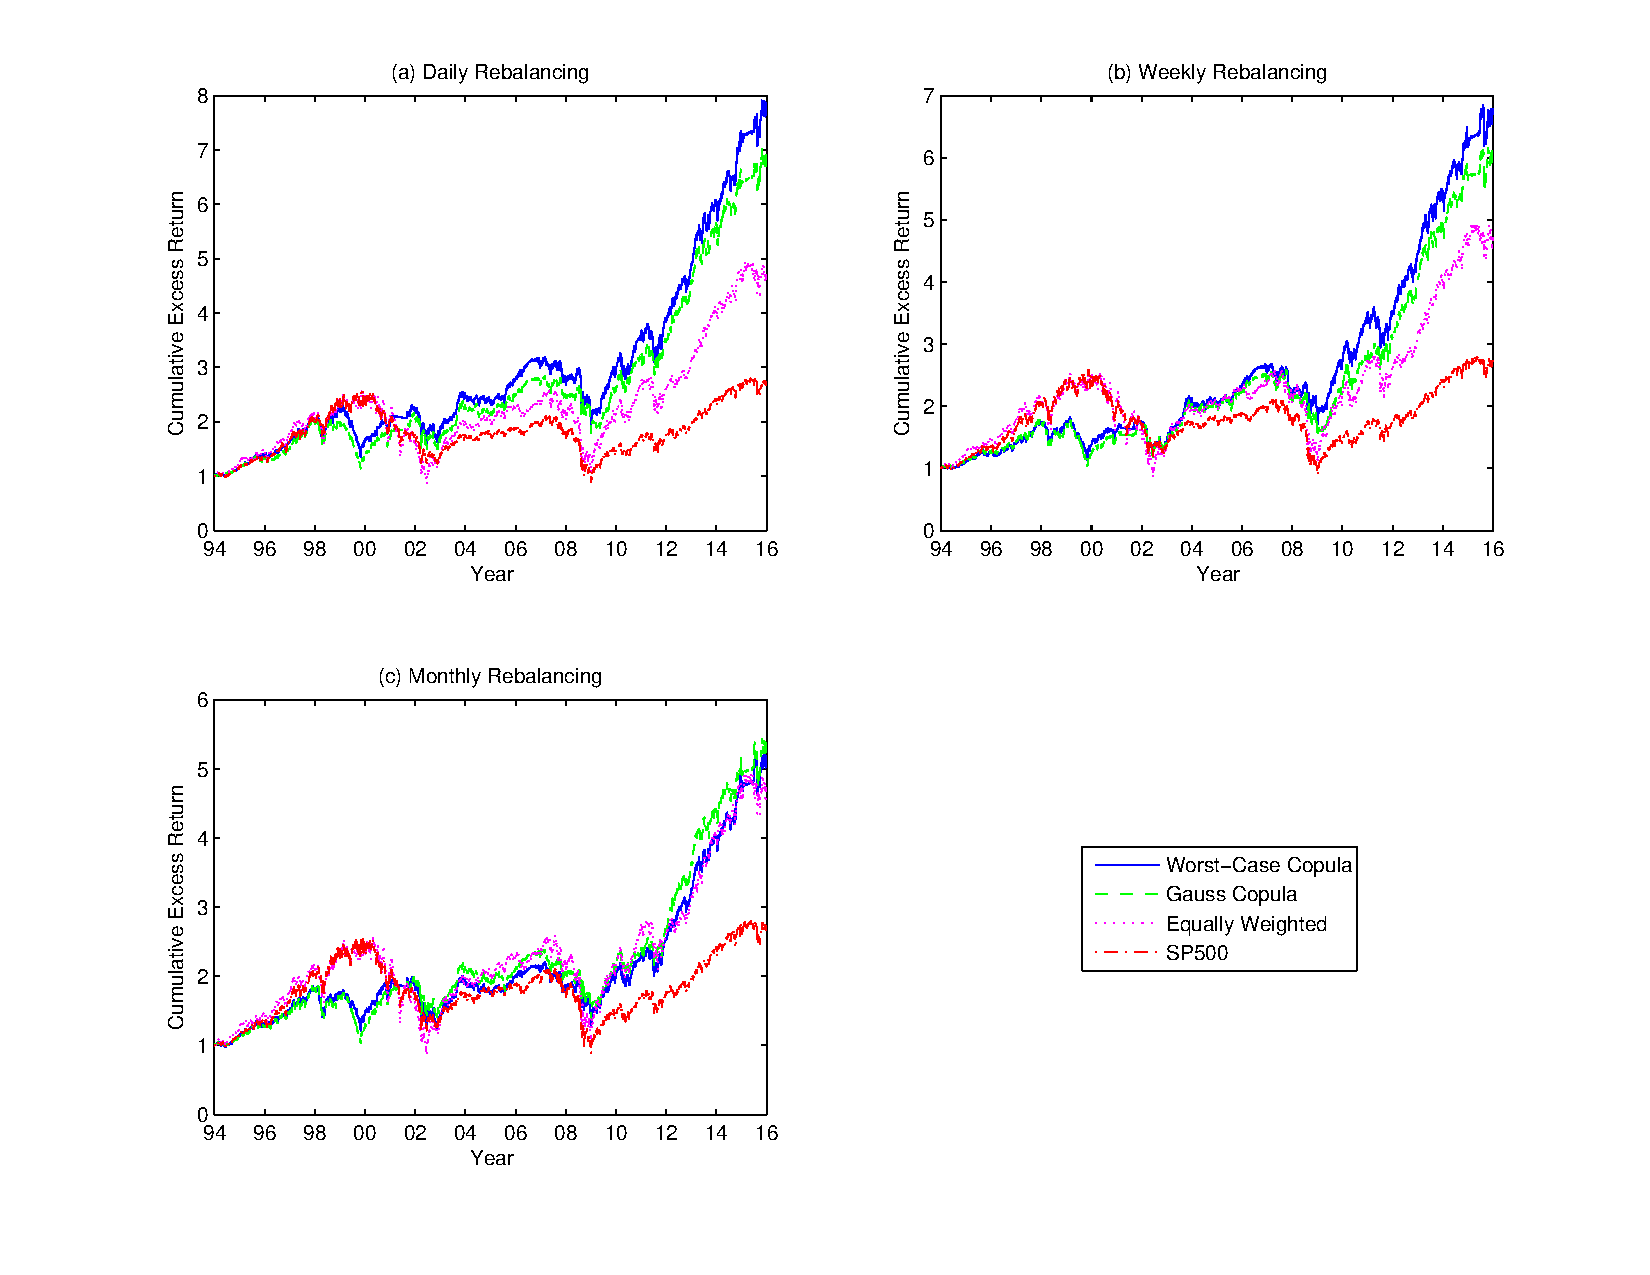
\includegraphics[scale=0.7]{fig1_nogrid.pdf}
	\caption{\scriptsize Cumulative excess returns of the portfolio strategies without daily target mean return }
	\caption*{This figure shows how an investment of \$1 evolves from July 1994 to December 2015 for every portfolio.}
	\label{fig:fig01}
\end{figure}

The copula-based approaches are more profitable for daily and weekly rebalancing over time, especially after 2009. Notice that the copula methods present a hump-shaped pattern in 1999, while the other benchmarks show a sharp decline in the subperiod that corresponds to the bear market that comprises the dotcom crisis and the September 11th terrorist attack (2000-2002). All portfolios show a hump-shaped pattern during the subprime mortgage financial crisis in 2007-2008. Overall, we can observe that after 2002 the patterns are similar, but the figure indicates that the copula methods, even though the objective function is the minimization of CVaR under a constraint on expected return, preserve more wealth in the long-term period, particularly the WCCVaR portfolio, for daily and weekly rebalancing \footnote{Transaction costs should not be neglected, corroborating our results from the breakeven analysis.}.

\section{Conclusions}

 In this paper, we combine robust portfolio optimization and copula-based models in a Worst Case CVaR framework. To cope with the large number of financial instruments, we employ a procedure similar to that used by \citet{ggr06} to select a set of diversified assets that can be useful during crises and tranquil periods. Using data from the S\&P 500 stocks from 1990 to 2015, we evaluate the performance of the WCCVaR (Worst Case Copula-CVaR) portfolio, considering different rebalancing strategies, and compare it to three benchmarks: a Gaussian Copula-CVaR (GCCVaR) portfolio, an equally weighted portfolio ($1/N$) and the S\&P 500 index. 

By selecting a diversified set of assets over a long-term period, we found that copula-based approaches offer better hedges against losses than the $1/N$ portfolio. Moreover, the WCCVaR approach generates portfolios with better downside risk statistics for any rebalancing period and are more profitable than the Gaussian Copula-CVaR for daily and weekly rebalancing.

Further studies should investigate the method of asset selection using nonlinear dependence measures between random variables of arbitrary dimensions \citep{lopez2013randomized} or procedures based on data mining tools as random forest \citep{dlrz10}. Additional suggestions include relaxing the assumption of no short selling and incorporate transaction cost as an additional constraint in the optimization problem as in \citet{krokhmal2002}.

\addcontentsline{toc}{section}{References}
\bibliographystyle{rfs}
\bibliography{mypapers}
\newpage

\end{document}
